% Generated by tools/figures.mjs from analysis/position-adjust-6model-2026-10-09.json and analysis/position-adjust-batchb-2026-10-09.json - do not edit by hand.
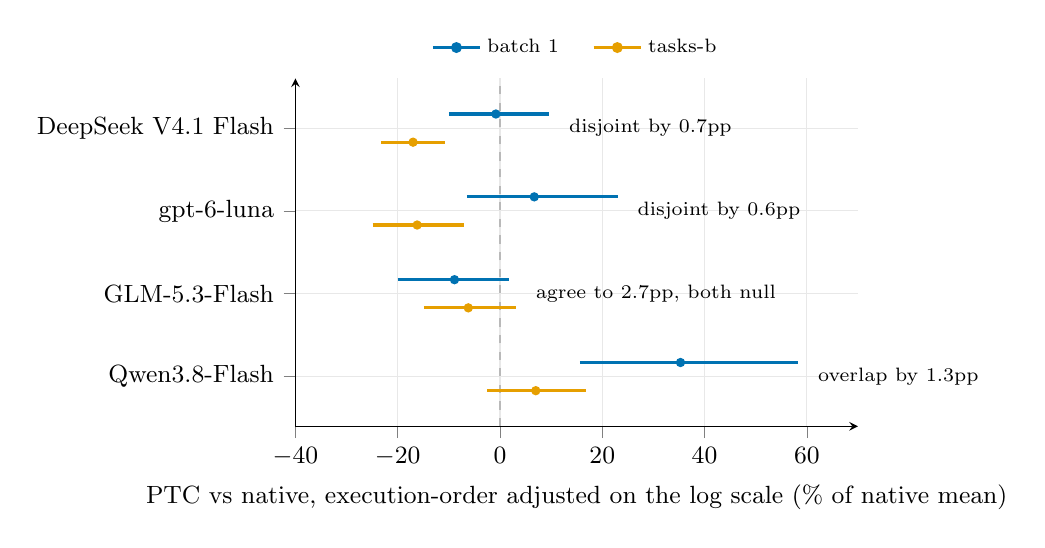
\begin{tikzpicture}
\definecolor{f2a}{HTML}{0072B2}
\definecolor{f2b}{HTML}{E69F00}
\begin{axis}[
  width=\linewidth-3.4cm, height=6.0cm, compat=1.18,
  xlabel={PTC vs native, execution-order adjusted on the log scale (\% of native mean)},
  xmin=-40, xmax=70,
  ytick={0,1,2,3},
  yticklabels={Qwen3.8-Flash,GLM-5.3-Flash,gpt-6-luna,DeepSeek V4.1 Flash},
  ymin=-0.6, ymax=3.60,
  axis y line=left, axis x line=bottom, tick align=outside,
  grid=major, grid style={gray!18},
  yticklabel style={font=\small}, xticklabel style={font=\small}, xlabel style={font=\small}, ylabel style={font=\small},
  legend style={at={(0.5,1.03)}, anchor=south, legend columns=2, draw=none, font=\scriptsize, /tikz/every even column/.append style={column sep=10pt}},
  clip=false,
]
\addlegendimage{f2a, line width=1.1pt, mark=*, mark size=1.4pt}
\addlegendentry{batch 1}
\addlegendimage{f2b, line width=1.1pt, mark=*, mark size=1.4pt}
\addlegendentry{tasks-b}
\draw[gray!55, dashed] (axis cs:0,-0.6) -- (axis cs:0,3.60);
\draw[f2a, line width=1.1pt] (axis cs:15.6,0.17) -- (axis cs:58.3,0.17);
\node[circle, fill=f2a, inner sep=1.2pt] at (axis cs:35.3,0.17) {};
\draw[f2b, line width=1.1pt] (axis cs:-2.5,-0.17) -- (axis cs:16.9,-0.17);
\node[circle, fill=f2b, inner sep=1.2pt] at (axis cs:7.0,-0.17) {};
\node[font=\scriptsize, anchor=west] at (axis cs:60.3,0) {overlap by 1.3pp};
\draw[f2a, line width=1.1pt] (axis cs:-20.0,1.17) -- (axis cs:1.8,1.17);
\node[circle, fill=f2a, inner sep=1.2pt] at (axis cs:-8.9,1.17) {};
\draw[f2b, line width=1.1pt] (axis cs:-14.9,0.83) -- (axis cs:3.1,0.83);
\node[circle, fill=f2b, inner sep=1.2pt] at (axis cs:-6.2,0.83) {};
\node[font=\scriptsize, anchor=west] at (axis cs:5.1,1) {agree to 2.7pp, both null};
\draw[f2a, line width=1.1pt] (axis cs:-6.5,2.17) -- (axis cs:23.0,2.17);
\node[circle, fill=f2a, inner sep=1.2pt] at (axis cs:6.7,2.17) {};
\draw[f2b, line width=1.1pt] (axis cs:-24.9,1.83) -- (axis cs:-7.1,1.83);
\node[circle, fill=f2b, inner sep=1.2pt] at (axis cs:-16.2,1.83) {};
\node[font=\scriptsize, anchor=west] at (axis cs:25.0,2) {disjoint by 0.6pp};
\draw[f2a, line width=1.1pt] (axis cs:-10.0,3.17) -- (axis cs:9.6,3.17);
\node[circle, fill=f2a, inner sep=1.2pt] at (axis cs:-0.8,3.17) {};
\draw[f2b, line width=1.1pt] (axis cs:-23.2,2.83) -- (axis cs:-10.8,2.83);
\node[circle, fill=f2b, inner sep=1.2pt] at (axis cs:-17.0,2.83) {};
\node[font=\scriptsize, anchor=west] at (axis cs:11.6,3) {disjoint by 0.7pp};
\end{axis}
\end{tikzpicture}
